 % PrivateMsg




  %% Old: Once the ordered set of constraints is defined, we discuss the idea of introducing an additional constraint to the set. The introduction of an additional constraint is problematic because it can hide or render irrelevant constraints that already exist in the set. However, by restricting the analysis to the \textit{relevant} set of constraints, we are able to

  %% Old: We now move on to the sources of consumption concavity. In our setting, there are two sources of consumption concavity: risk and constraints. The properties of consumption under risk have already been derived in \citet{carroll&kimball:concavity}. We therefore restrict our attention to showing how liquidity constraints make the consumption function concave. Once the relationship between liquidity constraints and consumption concavity is established, we use the results on consumption concavity and prudence to show under which conditions liquidity constraints heighten prudence.

  \subsection{Liquidity Constraints and Kink Points}\label{sec:LCandKinks}
  Recall that we are working with a consumer whose horizon goes from $0$ to $T$. We define a liquidity constraint dated $t$ as a constraint that requires savings at the \textit{end of period} $t \in (0, T]$ to be non-negative (the assumption of non-negativity is without loss of generality as shown in Theorem \ref{thm:lcip2}).


  We first define what we mean by a kink point which is induced by a constraint. To have a distinct terminology for the effects of current-period and future-period constraints, we will use the word `binds' to refer to the potential effects of a constraint in the period in which it applies and will use the term `impinges' to describe the effect of a future constraint on current consumption.
  \begin{defn}(Kink Point.) \\
    We define a kink point, $\wAlt_{t,n}$ as the level of market resources at which constraint $n$ stops binding or impinging on time $t$ consumption.
  \end{defn}
  \noindent A kink point corresponds to a transition from a level of market resources where a current constraint binds or a future constraint impinges, to a level of market resources where that constraint no longer binds or impinges.


  The timing of a constraint relative to other existing constraints matters for the effects of the constraint. We therefore define an ordered set to keep track of the existing constraints.
  \begin{defn} (An Ordered Set of Relevant Constraints.) \\
    We define $\mathcal{T}$ as an ordered set of dates at which a relevant constraint exists. We define $\mathcal{T}[1]$ as the last period in which a constraint exists, $\mathcal{T}[2]$ as the date of the last period before $\mathcal{T}[1]$ in which a constraint exists, and so on.
  \end{defn}
  \noindent $\mathcal{T}$ is the set of relevant constraints, ordered from the last to the first constraint. We order them from last to first because a constraint in period $t$ only affects behavior prior to period $t$ (and $t$ itself). The set of constraints from period $t$ to $T$ summarizes all relevant information in period $t$. Further, and as discussed below, the effect of imposing the next constraint in $\mathcal{T}$ on consumption is unambiguous only if one imposes constraints chronologically from last to first (and all constraints are of the no-borrowing type).

  For any $t \in [0, T)$, we define $c_{t,n}$ as the optimal consumption function in period $t$ assuming that the first $n$ constraints in $\mathcal{T}$ have been imposed. For example, $c_{t,0}({m})$ is the consumption function in period $t$ when no constraint has been imposed, $c_{t,1}({m})$ is the consumption function in period $t$ after the chronologically last constraint has been imposed, and so on. $\Omega_{t,n}, V_{t,n}$, and other functions are defined correspondingly.



  \subsection{A Fixed Set of Constraints}\label{subsec:Piecewise}

  We first consider an initial situation in which a consumer is solving a perfect foresight optimization problem with a finite horizon that begins in period $t$ and ends in period $T$. The consumer begins with market resources ${m}_{t}$ and earns constant income ${y}$ in each period. Lemma \ref{lem:LcAndCc} shows how this consumer's behavior in period $t$ changes from an initial situation with $n\geq 0$ constraints to a situation in which $n+1$ liquidity constraints has been imposed.

  \begin{lemma}\label{lem:LcAndCc}(Liquidity Constraints Cause Counterclockwise Concavification.) \\
    Consider an agent who has a utility function with $u'> 0 $ and $u'' < 0$, faces constant income ${y}$, and is impatient ($\beta R < 1$). Assume that the agent faces a set $\mathcal{T}$ of $N$ relevant constraints. Then $c_{t,n+1}({m})$ is a counterclockwise concavification of $c_{t,n}({m})$ around $\wAlt_{t,n+1}$ for $n \leq N-1$.
  \end{lemma}

  \noindent See Appendix \ref{app:pfclc} for the proof. When we have an ordered set of constraints, $\mathcal{T}$, the introduction of the next constraint generates a counterclockwise concavification of the consumption function.









  \subsection{Additional Constraints}
  \label{subsec:IncreaseNumConstr}

  Lemma \ref{lem:LcAndCc} analyzes the case where there is a preordained set of constraints $\mathcal{T}$ which were applied sequentially in reverse chronological order. We now examine how behavior will be modified if we add a new date $\hat{\tau}$ to the set of dates at which the consumer is constrained.

  Call the new set of dates $\hat{\mathcal{T}}$ with $N+1$ constraints (one more constraint than before), and call the consumption rules corresponding to the new set of dates
  $\hat{c}_{t,1}$ through $\hat{c}_{t,N+1}$. Now call $m$ the
  number of constraints in $\mathcal{T}$ at dates strictly
  greater than $\hat{\tau}$.  Then note that that $\hat{c}_{\hat{\tau},m} =
  c_{\hat{\tau},m}$, because at dates after the date at which the new constraint (number $m+1$) is
  imposed, consumption is the same as in the absence of the new constraint.
  Now recall that imposition of the constraint at $\hat{\tau}$ causes a counterclockwise concavification of the consumption function around a new kink point, $\wAlt_{\hat{\tau},m+1}$. That is, $\hat{c}_{\hat{\tau},m+1}$ is a counterclockwise concavification of $\hat{c}_{\hat{\tau},m} = c_{\hat{\tau},m}$.

  The most interesting observation, however, is that behavior under constraints $\hat{\mathcal{T}}$ in periods strictly before $\hat{\tau}$ \textit{cannot} be described as a counterclockwise concavification of behavior under $\mathcal{T}$.  The reason is that the values of wealth at which the earlier constraints caused kink points in the consumption functions before period $\hat{\tau}$ will not generally correspond to kink points once the extra constraint has been added.

  \hypertarget{CurrConstrHidesFutKink}{}

  \begin{figure}[ht]
    {\centering 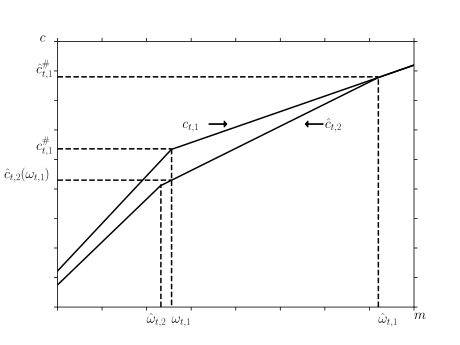
\includegraphics[width=.95\textwidth]{\FigDir/CurrConstrHidesFutKink}}
    \caption{How a future constraint can move a current kink}
    \footnotesize {\emph{Notes:} $c_{t,1}$ is the original consumption function with one constraint that induces a kink point at $\omega_{t,1}$. $\hat{c}_{t,2}$ is the modified consumption function in where we have introduced one new constraint. The two constraints affect $\hat{c}_{t,2}$ through two kink points: $\hat{\omega}_{t,1}$ and $\hat{\omega}_{t,2}$. Since we introduced the new constraint at a later point in time than the current existing constraint, the future constraint affects the position of the kink induced by the current constraint and the modified consumption function $\hat{c}_{t,2}$ is not a counterclockwise concavification of ${c}_{t,1}$.}
    \label{fig:LCtHidesLCtpn}
  \end{figure}

  Figure~\ref{fig:LCtHidesLCtpn} presents an example. The original $\mathcal{T}$ contains only a single constraint, at the end of period $t+1$, inducing a kink point at $\wAlt_{t,1}$ in the consumption rule $c_{t,1}$. The expanded set of constraints $\hat{\mathcal{T}}$ adds one constraint at period $t+2$. $\hat{\mathcal{T}}$ induces two kink points in the updated consumption rule $\hat{c}_{t,2}$, at $\hat{\wAlt}_{t,1}$ and $\hat{\wAlt}_{t,2}$.  It is true that imposition of the new constraint causes consumption to be lower than before at every level of wealth below $\hat{\wAlt}_{t,1}$.  However, this does not imply higher prudence of the value function at every ${m} <\hat{\wAlt}_{t,1}$.  In particular, the original consumption function is strictly concave at $\wAlt_{t,1}$, while the new consumption function is linear at $\wAlt_{t,1}$, so prudence is greater before than after imposition of the new constraint at $\wAlt_{t,1}$.

  The intuition is straightforward. At levels of initial wealth below $\hat{\wAlt}_{t,1}$, the consumer had been planning to end period $t+2$ with negative wealth. With the new constraint, the old plan of ending up with negative wealth is no longer feasible and the consumer will save more for any given level of current wealth below $\hat{\wAlt}_{t,1}$, including $\wAlt_{t,1}$. But the reason $\wAlt_{t,1}$ was a kink point in the initial situation was that it was the level of wealth where consumption would have been equal to market resources in period $t+1$. Now, because of the extra savings induced by the constraint in $t+2$, the period $t+1$ constraint will no longer bind for a consumer who begins period $t$ with wealth $\wAlt_{t,1}$. In other words, at wealth $\wAlt_{t,1}$ the extra savings induced by the new constraint prevents the original constraint from being relevant at $\wAlt_{t,1}$.

  Notice, however, that all constraints that existed in $\mathcal{T}$ will remain relevant at \textit{some} $m$ under $\hat{\mathcal{T}}$ even after the new constraint is imposed - they just induce kink points at different levels of market resources than before (in Figure \ref{fig:LCtHidesLCtpn}, the first constraint causes a kink at $\hat{\wAlt}_{t,2}$ rather than $\wAlt_{t,1}$).

  \subsection{A More General Analysis}
  \label{subsubsec:MoreGenConstr}
  The preceding analyses required income to be constant, the liquidity constraints to be of the no-borrowing type, and consumers to be impatient ($\beta R < 1$).  We now relax these requirements.
  %% Old: We now want to allow time variation in the level of income ${y}_{t}$ and in the location of the liquidity constraint .  We also drop the restriction that $\beta R < 1$, allowing the consumer to desire consumption growth over time.

  Under these more general circumstances, a constraint imposed in a given period can render constraints in either earlier or later periods irrelevant.  For example, consider a consumer with CRRA utility and $\beta R=1$ who earns income of 1 in each period, but who is required to arrive at the end of period $T-2$ with savings of 5.  Then a constraint that requires savings to be greater than zero at the end of period $T-3$ will have no effect because the consumer is required by the constraint in period $T-2$ to end period $T-3$ with savings greater than 4.

  Formally, consider now imposing the first constraint, which applies in period $\tau < T$.  The simplest case, analyzed before, was a constraint that requires the minimum level of end-of-period wealth to be ${a}_{\tau} \geq 0$.  Here we generalize this to ${a}_{\tau} \geq \sConst_{\tau,1}$ where in principle we can allow borrowing by choosing $\sConst_{\tau,1}$ to be a negative number. Now for constraint $1$ calculate the kink points for prior periods from
  \begin{eqnarray}
    u'(c_{\tau,1}^{\#}) & = & R\beta u'(c_{\tau+1,0}(R\sConst_{\tau,1}+{y}_{\tau + 1}))
    \\ \wAlt_{\tau,1} & = & (V_{\tau,1}')^{-1}(u'(c_{\tau,1}^{\#})).
  \end{eqnarray}
  In addition, for constraint $2$ recursively calculate
  \begin{eqnarray}
    \underline{\sConst}_{\tau-1,1} & = & (\sConst_{\tau,1}-{y}_{\tau,2}+\underline{c})/R  \label{eq:cgt0}
  \end{eqnarray}
  where $\underline{\sConst}_{\tau-1,1}$ is the level of wealth that constraint $1$ requires the agent to end period $\tau-1$ with and $\underline{c}$ is the lower bound for the value of consumption permitted by the model (independent of constraints).\footnote{For example, CRRA utility is well defined only on the positive real numbers, so for a CRRA utility consumer $\underline{c}=0$.  In other cases, for example with exponential or quadratic cases, there is nothing to prevent consumption of $-\infty$, so for those models $\underline{c}=-\infty$, unless there is a desire to restrict the model to positive values of consumption, in which case the $c\geq 0$ constraint will be implemented through the use of \eqref{eq:cgt0}.}

  Now assume that the first $n$ constraints in $\mathcal{T}$ have been imposed, and consider imposing constraint number $n+1$, which we assume applies at the end of period $\tau$.  The first thing to check is whether constraint number $n+1$ is relevant given the already-imposed set of constraints. This is simple: A constraint that requires ${a}_{\tau} \geq \sConst_{\tau,n+1}$ will be irrelevant if $\max_{i \in [1,n]} [\underline{\sConst}_{\tau,i}] \geq \sConst_{\tau,n+1}$, i.e.\ if one of the existing constraints already implies that savings must be greater or equal to value required by the new constraint.  If the constraint is irrelevant then the analysis proceeds simply by dropping this constraint and renumbering the constraints in $\mathcal{T}$ so that the former constraint $n+2$ becomes constraint $n+1$, $n+3$ becomes $n+2$, and so on.

  Now consider the other possible problem: That constraint number $n+1$ imposed in period $\tau$ will render irrelevant some of the constraints that have already been imposed.  This too is simple to check: It will be true if the proposed $\sConst_{\tau,n+1} \geq \sConst_{\tau,i}$ for any $i \leq n$ and for all ${m}$.\footnote{If a constraint is irrelevant for the lowest ${m}$ that t could enter period $\tau$ with, then it is irrelevant for all ${m}$.} The fix is again simple: Counting down from $i=n$, find the smallest value of $i$ for which $\sConst_{\tau,n+1} \geq \sConst_{\tau,i}$.  Then we know that constraint $n+1$ has rendered constraints $i$ through $n$ irrelevant. The solution is to drop these constraints from $\mathcal{T}$ and start the analysis over again with the modified $\mathcal{T}$.

  If this set of procedures is followed until the chronologically earliest relevant constraint has been imposed, the result will be a $\mathcal{T}$ that contains a set of constraints that can be analyzed as in the simpler case. In particular, proceeding from the final $\mathcal{T}[1]$ through $\mathcal{T}[N]$, the imposition of each successive constraint in $\mathcal{T}$ now causes a counterclockwise concavification of the consumption function around successively lower values of wealth as progressively earlier constraints are applied and the result is again a piecewise linear and strictly concave consumption function with the number of kink points equal to the number of constraints that are relevant at any feasible level of wealth in period $t$.

  The preceding discussion establishes the following result:

  \begin{theorem}\label{thm:lcip2} (Liquidity Constraints Cause Counterclockwise Concavification.) \\
    Consider an agent in period $t$ who has a utility function with $u' > 0$, $u'' < 0$, $u''' \geq 0$, and non-increasing absolute prudence ($-u'''/u''$). Assume that the agent faces a set $\mathcal{T}$ of $N$ relevant constraints.  Then $c_{t,n+1}({m})$ is a counterclockwise concavification of $c_{t,n}({m})$ around $\wAlt_{t,n+1}$.
    %	When $n \leq N-1$ constraints have been imposed, the imposition of constraint $n+1$ strictly increases absolute prudence of the agent's value function if the utility function satisfies $u''' > 0$ and ${m}_{t} < \wAlt_{t,n+1}$ or if $u''' = 0$ and $\frac{c'_{t,n+1}}{c'_{t,n}}$ strictly declines at ${m}$.
  \end{theorem}



  %% Old: \begin{theorem}\label{thm:lcip2} (Liquidity Constraints Increase Prudence.) \\
  %%   Old:   Consider an agent in period $t$ who has a utility function with $u' > 0$, $u'' < 0$, $u''' \geq 0$, and non-increasing absolute prudence ($-u'''/u''$). Assume that the agent faces a set $\mathcal{T}$ of $N$ relevant constraints. When $n \leq N-1$ constraints have been imposed, the imposition of constraint $n+1$ strictly increases absolute prudence of the agent's value function if the utility function satisfies $u''' > 0$ and ${m}_{t} < \wAlt_{t,n+1}$ or if $u''' = 0$ and $\frac{c'_{t,n+1}}{c'_{t,n}}$ strictly declines at ${m}$.
  %%   Old: \end{theorem}

  \noindent Theorem \ref{thm:lcip2} is a generalization of Lemma \ref{lem:LcAndCc}. Even if we relax the assumptions that income is constant and the agent is impatient, the imposition of an extra (more general) constraint increases absolute prudence of the value function as long as we are careful when we select the set $\mathcal{T}$ of relevant constraints.

  For an agent that only faces liquidity constraints, but no risk, the shape of the consumption function is piecewise linear.
  %% Old: \begin{corollary}(Piecewise Linear Consumption Function.) \\
  %%   Old:   Consider an agent who has a utility function with $u'> 0$ and $u'' < 0$, faces constant income ${y}$, and is impatient. Assume that the agent faces a set $\mathcal{T}$ of $N$  constraints. When $n \leq N$ constraints have been imposed, $c_{t,n}({m})$ is a piecewise linear increasing concave function with kink points at successively larger values of wealth at which future constraints stop impinging on current consumption.
  %%   Old: \end{corollary}
  Since the consumption function is piecewise linear, the new consumption function, $c_{t,n+1}({m})$ is not necessarily strictly more concave than $c_{t,n}({m})$ for all ${m}$. This is where the concept of counterclockwise concavification is useful. Even though $c_{t,n+1}({m})$ is not strictly more concave than $c_{t,n}({m})$ everywhere, it is a counterclockwise concavification and we can apply Lemma \ref{lem:CCToPrud} and \ref{lem:ccandstrictprud} to show that the introduction of the next liquidity constraint increases absolute prudence of the value function.

  \begin{corollary}\label{cor:lcip} (Liquidity Constraints Increase Prudence.) \\
    Consider an agent in period $t$ who has a utility function with $u' > 0$, $u'' < 0$, $u''' \geq 0$, and non-increasing absolute prudence ($-u'''/u''$). Assume that the agent faces a set $\mathcal{T}$ of $N$ relevant constraints. When $n \leq N-1$ constraints have been imposed, the imposition of constraint $n+1$ strictly increases absolute prudence of the agent's value function if the utility function satisfies $u''' > 0$ and ${m}_{t} < \wAlt_{t,n+1}$ or if $u''' = 0$ and $\frac{c'_{t,n+1}}{c'_{t,n}}$ strictly declines at ${m}$.
  \end{corollary}
  \begin{proof}
    By Theorem \ref{thm:lcip2}, the imposition of constraint $n+1$ constitutes a counterclockwise concavification of $c_{t,n}({m})$. By Lemma \ref{lem:CCToPrud} and \ref{lem:ccandstrictprud}, such a concavification (strictly) increases absolute prudence of the value function.
  \end{proof}
  \noindent %In the subsequent discussions, we consider cases where we relax the assumptions underlying Corollary \ref{cor:lcip}. We first consider the case where we add an extra constraint to the set of constraints. Next, we consider the cases with time-varying deterministic income, general constraints, and no assumption on time discounting.

  %% Old: Finally, consider adding a new constraint to the problem and call the new set of constraints $\hat{\mathcal{T}}$.  Suppose the new constraint applies in period $\hat{\tau}$.  Then the analysis of the new situation will be like the analysis of an added constraint in the simpler case in section \ref{subsec:IncreaseNumConstr} if the new constraint is relevant given the constraints that apply after period $\hat{\tau}$ and the new constraint does not render any of those later constraints irrelevant. If the new constraint fails either of these tests, the analysis of $\hat{\mathcal{T}}$ can proceed from the ground up as described above.


  \newpage
